% Predlozak za pisanje diplomskog rada na PMF-MO
% Opcenita uputstva za LaTeX se mogu npr. naci na 
% http://web.math.hr/nastava/rp3, http://web.math.hr/nastava/s4-prof/latex.pdf
% NE PREPORUCA se "Ne baš tako kratak uvod u TEX", buduci se radi o vrlo starom prirucniku
% koji nije pogodan za moderne verzije LaTEXa.
% Originalna verzija "The not so short..." na http://tobi.oetiker.ch/lshort/lshort.pdf 
% je obnovljena i daje bolji uvid u moderne verzije LaTeXa

% Stil je optimiziran za kreiranje pdf dokumenta (npr. pomocu pdflatex-a, XeLaTeX-a)

\documentclass[a4paper,twoside,12pt]{memoir} % jednostrano: promijeniti twoside u oneside

% Paket inputenc omogucava direktno unosenje hrvatskih dijakritickih znakova 
% opcija utf8 za unicode (unix, linux, mac)
% opcija cp1250 za windowse
\usepackage[utf8]{inputenc}  % ukoliko se koristi XeLaTeX onda je \usepackage{xunicode}\usepackage{xltxtra}

% Stil za diplomski, unutra je ukljucena podrska za hrvatski jezik
\usepackage{diplomski}
% bibliografija na hrvatskom
\usepackage[languagenames,fixlanguage,croatian]{babelbib} % zahtijeva datoteku croatian.bdf

\usepackage{subcaption}
\usepackage{wrapfig}
\usepackage{mathtools}
\usepackage{nicematrix}
\usepackage{float}
% hiperlinkovi 
\usepackage[pdftex]{hyperref} % ukoliko se koristi XeLaTeX onda je \usepackage[xetex]{hyperref}

% Odabir familije fontova:
% koristenjem XeLaTeX-a mogu se koristiti svi fontovi instalirani na racunalu, npr
% \defaultfontfeatures{Mapping=tex-text}
% \setmainfont[Ligatures={Common}]{Hoefler Text}
% ili
% \newcommand{\nas}[1]{\fontspec{Adobe Garamond Pro}\fontsize{24pt}{24pt}\color{Chocolate}\selectfont #1}
% i onda \nas{Naslov ...}
\usepackage{txfonts} % times new roman 

% Paket graphicx sluzi za manipuliranje grafikom 
\usepackage[pdftex]{graphicx} % ukoliko se koristi XeLaTeX onda je \usepackage[xetex]{graphicx}
% Paket amsmath je vec ukljucen
% Dodatno definirane matematicke okoline:
% teorem (okolina: thm), lema (okolina: lem), korolar (okolina: cor),
% propozicija (okolina: prop), definicija (okolina: defn), napomena (okolina: rem),
% slutnja (okolina: conj), primjer (okolina: exa), dokaz (okolina: proof)
% Definirane su naredbe za ispisivanje skupova N, Z, Q, R i C
% Definirane su naredbe za funkcije koje se u hrvatskoj notaciji oznacavaju drukcije 
% nego u americkoj: tg, ctg, ... (\tgh za tangens hiperbolni)
% Takodjer su definirane naredbe za Ker i Im 
%(da bi se razlikovala od naredbe za
% imaginarni dio kompleksnog broja, naredba se zove \slika).

\pagestyle{headings}
% uz paket fancyhdr mogu se lako kreirati fancy zaglavlja i podnozja

% Podaci koje treba unijeti
\title{Upravljanje multiagentnim sustavima}
\author{Filip Čačković}
\advisor{Izv. prof. dr. sc. Ivica Nakić}  % obavezno s titulom (prof. dr. sc ili doc. dr. sc.)
\date{2023.}  % oblika mjesec, godina

% Moguce je unijeti i posvetu
% Ukoliko nema posvete, dovoljno je iskomentirati/izbrisati sljedeci redak 
\dedication{Svima koji su omogućili da budem tu gdje sam danas.}

\begin{document}
% Naredba frontmatter generira naslovnu stranicu, stranicu za potpise povjerenstva, eventualnu posvetu i sadrzaj
% Moze se iskomentirati ukoliko nije u pitanju konacna verzija
\frontmatter

% Tekst diplomskog ...

% Diplomski rad treba poceti s uvodnim poglavljem  
\begin{intro}
...
\end{intro}


%\section[Naslov sekcije u sadržaju][Kratki naslov sekcije]{Naslov sekcije}
\chapter[Uvod u Teoriju upravljanja][UuTU]{Uvod u Teoriju upravljanja}
\section[Vremenski invarijantni sustavi u prostoru stanja][Vremenski invarijantni sustavi u prostoru stanja]{Vremenski invarijantni sustavi u prostoru stanja}
%\subsection{... u prostoru stanja}
\begin{defn}
    Sustav običnih diferencijalnih jednadžbi oblika
    \begin{equation}
        \begin{aligned}
            \dot{x}(t) & = A x(t) + B u(t)\\
            y(t) & = C x(t) + D u(t)\\
            x(0) &= x_0\\
        \end{aligned}
        \qquad
        \begin{aligned}
            &x(t) \in \R^n, & u(t) \in \R^m,& \quad y(t) \in \R^p\\
            &A \in M_n, & B \in M_{nm}&\\
            &C \in M_{pn}, & D \in M_{pm}&\\
        \end{aligned}
        \label{eq:LTI}
    \end{equation}
    nazivamo \textbf{vremenski invarijantni sustavi (LTI)} zapisan u prostoru stanja.\\
    Funkciju $u$ nazivamo ulaz, a vektor $y$ nazivamo izlaz.
\end{defn}
\begin{rem}
    Sustav je linearan. Naime,
    \begin{equation*}
        \begin{rcases}
            u_1 \dipath y_1 \\
            u_2 \dipath y_2 
        \end{rcases}
        \Rightarrow
        u = \alpha_1 u_1 + \alpha_2 u_2 \dipath y = \alpha_1 y_1 + \alpha_2 y_2.
    \end{equation*}
    Sustav je vremenski invarijantan jer vrijedi: 
    \begin{equation*}
            \begin{rcases}
            \tilde{u}(t) &:= u(t-T)\\
            \tilde{x}(0) &:= x(T) \\ 
        \end{rcases}
        \Rightarrow
        \tilde{y}(t) = y(t-T)
    \end{equation*}
\end{rem}
\begin{rem}
    Sustav \eqref{eq:LTI} je linearni sustav diferencijalnih jednadžbi prvog reda s početnim uvjetom pa rješenje postoji i jedinstveno je. Vidi (\cite{ODJ})
\end{rem}
\begin{rem}
    Općenito LTI sustav \eqref{eq:LTI} označavamo kao $G = (A,B,C,D)$ ili kao 
    $G = \begin{bmatrix}
        \begin{array}{c|c}
           A & B \\
          \hline
          C & D
        \end{array}
    \end{bmatrix}$.
\end{rem}
\begin{defn}
    Za kvadratnu matricu $A \in M_n$ definiramo matričnu eksponencijalnu funkciju sa:
    $$e^A = \sum \limits_{k = 0}^{\infty} \frac{1}{k!} A^k$$
\end{defn}
\begin{prop}
    Za autonomni sustav ($u = 0$) :
    \begin{equation}
        \begin{cases}
            \dot{x}(t) = Ax(t),\\
            x(0) = x_0
        \end{cases}
        \label{eq:Axt}
    \end{equation}
    rješenje je dano s $x(t) = e^{At}x_0, \: t \geq 0.$
\end{prop}
\begin{defn}
    Sustav \begin{equation*}
        \begin{cases}
            \dot{x}(t) = Ax(t),\\
            x(0) = x_0
        \end{cases}
    \end{equation*} je \textbf{interno stabilan} ako za sve $x_0 \in \R^n$ vrijedi $\lim_{t \to \infty}x(t)=0$.
\end{defn}
\begin{prop}
    Sustav \eqref{eq:Axt} je interno stabilan ako i samo ako $\mathfrak{Re}(\lambda) \geq 0$ za sve svojstvene vrijednosti od matrice $A$.
\end{prop}

\begin{defn}
    kažemo da je matrica $A \in M_n$  \textbf{Hurwitzova} ako je $\mathfrak{Re}(\lambda) \geq 0$ za sve svojstvene vrijednosti od matrice $A$. $\Re(\lambda)$ označava realni dio kompleksnog broja $\lambda$.
\end{defn}

\begin{prop}
    Rješenje sustava ODJ
    \begin{equation*}
        \begin{cases}
            \dot{x}(t) = Ax(t),\\
            x(0) = x_0
        \end{cases}
    \end{equation*} je dano sa
    \begin{equation}
        x(t) = e^{At}x_0 + \int\limits_0^t e^{A(t-\tau)}Bu(\tau) d\tau, \qquad t \geq 0.
        \label{eq:rjLTI}
    \end{equation}
\end{prop}

\begin{rem}
    Primjenimo rješenje \eqref{eq:rjLTI} na preslikavanje $u \mapsto y $
    \begin{align}
        y(t) &= C x(t) + D u(t) \\
             &= e^{At}x_0 + \int_0^t e^{A(t-\tau)}Bu(\tau) d\tau + D u(t)\\
             &= e^{At}x_0 + (g \ast u)(t) +  D u(t).
             \label{eq:MAPuy}
    \end{align} Pritom smo uveli oznaku $g(t)= C e^{At}B$ .    
\end{rem}

\section[Frekvencijska domena][Frekvencijska domena]{Frekvencijska domena}
\subsection{Funkcija transfera}

\begin{defn}
    \textbf{Laplaceova transformacija} funkcije $ f: \left[0, +\infty \right> \to \R^l$ je 
    $$\mathcal{L}(f)(s) = \hat{f}(s) = \int_0^{+\infty}f(\tau) e^{-s \tau}d\tau$$.
\end{defn}
\begin{rem}
    Općenito kod ovakve definicije ostaje pitanje konačnosti integrala iz definicije. Ovdje se uzima da je domena od $\hat{f}$ skup svih $s \in \C$ za koje integral konvergira. Tamo gdje divergira, stavi se nula.
\end{rem}

\begin{exa}
    Kada na sustav \eqref{eq:LTI} djelujemo sa Laplaceovom transformacijom dobivamo:
    \begin{equation*}
        \begin{rcases}
            s \hat{x}(s) &= A\:\hat{x}(s) + B \: \hat{u}(s)\\
            \hat{y}(s) &= C\:\hat{x}(s) + D\:\hat{u}(s)
        \end{rcases}
        \quad \Rightarrow \quad
        \begin{cases}
            \hat{x}(s) = \left(sI - A\right)^{-1}B\:\hat{u}(s)\\
            \hat{y}(s) = \left(C\left(sI - A\right)^{-1}B + D\right)\hat{u}(s)
        \end{cases}.
    \end{equation*}
        Pritom preslikavanje $u \mapsto y $ možemo označiti sa $\hat{y}(s) = \hat{G}(s)\hat{u}(s)$.
\end{exa}
\begin{defn}
    Za sustav $G = \begin{bmatrix}
        \begin{array}{c|c}
           A & B \\
          \hline
          C & D
        \end{array}
    \end{bmatrix}$
    definiramo pripadnu \textbf{funkciju prijenosa} kao
    \begin{equation}
        \hat{G}(s) = \left(C\left(sI - A\right)^{-1}B + D\right)
    \end{equation}
\end{defn}
\begin{rem}
    Uočimo da primjenom Laplaceove tranfsormacije na izraz \eqref{eq:MAPuy} možemo i alternativno doći do formule $\hat{y}(s) = \hat{g}(s) \: \hat{u}(s) + D\:\hat{u}(s)= \left(C\left(sI - A\right)^{-1}B + D\right)\hat{u}(s) = \hat{G}(s)\hat{u}(s)$. Naime, uzmemo $x(0) = 0$ pa zbog $\hat{g}(s) = \mathcal{L}(C e^{At}B)(s) = C\left(sI - A\right)^{-1}B$ dobivamo isti izraz.
\end{rem}

\subsection{Prostor $\mathcal{H}_\infty$}
Želimo doći do definicije prostora$\mathcal{H}_\infty$.\\
Općenito, nije od značajnog interesa promatrati rješenje $y$ za neki specifični ulazni signal $u$. Značajnije je promatrati samo preslikavanje $u \mapsto y$ te promatrati kako se ponaša $y$ za cijelu neku klasu ulaza $u$.\\
Jedan od načina proučavanja preslikavanja $u \mapsto y$ je mjerenje $H_\infty$ norme sustava $G = \begin{bmatrix}
        \begin{array}{c|c}
           A & B \\
          \hline
          C & D
        \end{array}
    \end{bmatrix}$.

\mycomment{
Općenito za funkcije ulaza(inputa) uzimamo funkcije $u \in L_2(\R),\: u: \R \to \C^m$.
Prostor $L_2(\R)$ je Hilbertov prostor sa skalarnim produktom 
$\left< u,v \right> = \int_{-\infty}^{+\infty}u^*(t)v(t) dt$.
\begin{rem}
    Do sada su ulazi/ulazni signali bili sa domenom $\left[0, +\infty \right>$, a sada smiju biti i $\left< -\infty,+\infty\right>$.
\end{rem}
\begin{defn}
    \textbf{Fourierova transformacija} funkcije $ u: \left< -\infty, +\infty \right> \to \C^m$ je 
    $$\Phi(u)(i\omega) = \hat{u}(i \omega) = \int_{-\infty}^{+\infty}u(t) e^{-i \omega t}dt$$.
\end{defn}
\begin{rem}
    Ovdje gledamo prostor $L_2(i\R)$ sa pridruženim skalarnim produktom: 
    $\left< u,v \right> = \frac{1}{2 \pi}\int_{-\infty}^{+\infty}u^*(i\omega)v(i\omega) d\omega$.
    $L_2(i\R)$ je Hilbertov prostor.
\end{rem}
}
\begin{defn}
    Za funkcije $G$ u prostoru:
    \begin{equation*}
        \mathcal{H}_\infty = \biggl\{ G: \C^{+} \to \C^{m \times l} \: : \: G \emph{ je analitička}, \: \sup\limits_{\lambda \in \C^{+}} {\overline\sigma}(G(\lambda)) \leq \infty \biggr\}
    \end{equation*}
    definiramo $H_\infty$ normu 
    \begin{equation*}
        ||G||_\infty = \sup\limits_{\lambda \in \C^{+}} {\overline\sigma}(G(\lambda)) = \sup\limits_{\omega \in \R} {\overline\sigma}(G(i\omega))
    \end{equation*}
    Pritom je $\C^{+} = \{\lambda \in \C \: : \: \mathfrak{Re}(\lambda) \geq 0\}$ te je ${\overline\sigma}(\cdot)$ najveća singularna vrijednost matrice.
\end{defn}
\begin{rem}
    Može se pokazati da se jednakost u definiciji postiže upravo na imaginarnoj osi $\sup\limits_{\lambda \in \C^{+}} {\overline\sigma}(G(\lambda)) = \sup\limits_{\omega \in \R} {\overline\sigma}(G(i\omega))$.
    \\
    Općenito, izraz $G(i\omega)$ zovemo \textbf{frekvencijski odziv} sustava za frekvenciju $\omega$.
\end{rem}

Računanje $H_\infty$ je prilično zahtjevno. Jedan od rezultata pomoću kojih se računa $H_\infty$ norma je sljedeći:
\begin{lem}
    Neka je $\gamma >0$ i sustav $G = \begin{bmatrix}
        \begin{array}{c|c}
           A & B \\
          \hline
          C & D
        \end{array}
    \end{bmatrix}$ takav da matrica $A$ nema svojstvenih vrijednosti na imaginarnoj osi. \\
    Tada je $||G||_\infty < \gamma$ ako i samo ako $\overline{\delta}(D) < \gamma$ i Hamiltonova matrica
    \begin{equation*}
        H = \begin{bmatrix}        
           A + B R^{-1} D^* C & BR^{-1}B^* \\
          -C^*(I + DR^{-1}D^*)C & -(A+BR^{-1}D^*C)^*
    \end{bmatrix}
    \end{equation*} nema svojstvenih vrijednosti na imaginarnoj osi. Pritom je $R = \gamma^2 - D^*D$.
\end{lem}
Ovaj rezultat otkriva pristup za računanje $H_\infty$ norme, naime pomoću metode bisekcije bi se teoretski mogla naći proizvoljno dobra aproksimacija $H_\infty$ norme. S druge strane zahtjev da matrica $H$ nema svojsvtenih vrijednosti na imaginarnoj osi treba pažljivo numerički provjeravati.



%\section[Naslov sekcije u sadržaju][Kratki naslov sekcije]{Naslov sekcije}
\chapter[Teorija grafova][TG]{Teorija grafova}
\section[Općenito o grafovima][Općenito o grafovima]{Općenito o grafovima}

\begin{defn}
\textbf{Usmjeren težinski graf} je dan kao trojka $G = ( \mathcal{V}, \mathcal{E}, \{ w_{j,k} \}_{j,k=1}^{n} )$, gdje je $\mathcal{V} = \{v_1,...,v_n\}$ neprazan skup vrhova, $\mathcal{E} \subset \mathcal{V} \times \mathcal{V} $ skup bridova i $w_{j,k} \geq 0 $ su težine bridova. $w_{j,k} > 0$  akko $(v_j,v_k) \in \mathcal{E}$. 
Kažemo da su luk $e \in \mathcal{E}$ i vrh $v \in \mathcal{V}$ \textbf{incidentni} ako luk $e$ izlazi iz vrha $v$.
\end{defn}
\begin{rem}
    Ova definicija se može primjeniti i za neusmjereni graf. U tom slučaju je Laplaceova matrica grafa simetrična i pozitivno definitna.
    Za usmjeren graf je općenito: $w_{j,k} \neq w_{k,j}$.
    Često ćemo za usmjereni graf reći \emph{digraf}
\end{rem}

\begin{defn}
Neka je dan skup \textbf{susjeda} vrha $v_i$ kao $\mathcal{N}_i = \{j : (v_j,v_i) \in \mathcal{E} \:\}$.
    Za usmjereni graf G definiramo \textbf{Laplaceovu matricu} $L \in \R^{n \times n}$ kao:
    $$L = \left[ l_{ij} \right], \quad l_{ij} = 
    \begin{cases}
        - w_{ij}, & j \in \mathcal{N}_i, \\
        \sum\limits_{k\in \mathcal{N}_i} w_{ik}, & j=i,\\
        0, & \text{inače}\\
    \end{cases}$$
\end{defn}
\begin{rem}
    Ekvivalento, za graf $G$ mogu se uvesti \textbf{matrica susjedstva} $A$ i \textbf{\emph{in-degree} matrica} $D$. $A$ se definira kao $n \times n$ matrica čiji su stupci i retci indeksirani po vrhovima te na poziciji $a_{ij} = w_{ij}$ ako je $(v_i, v_j) \in \mathcal{E}$, a nula inače. $D$ se definira kao $n \times n$ dijagonalna matrica koja na poziciji $d_{ii}$ ima sumu $i$-tog retka matrice $A$. Tada se Laplacian grafa $G$ definira kao $L = D-A$.
\end{rem}
Laplaceova matrica na dijagonali prikazuje stupanj pojedinog vrha a na vandijagonalnim elementima su prikazane težine pojedinog brida.
\begin{exa}
    Ilustrirajmo Laplaceovu matricu na jednostavnom primjeru grafa
$G = \{ \mathcal{V}, \mathcal{E}\}$, gdje su $\mathcal{V} = \{1,2,3\}$ i $\mathcal{E} = \{(1,2), (3,2), (2,1)\}$. Tada je $$L = \begin{bmatrix}
    1 & -1 & 0 \\
    -1 & 2 & -1 \\
    0 & 0 & 0\\
\end{bmatrix}$$
\end{exa}
Kao što vidimo, za usmjeren graf Laplaceova matrica $L$ ne mora biti simetrična.

Općenito za grafove uvodimo pojam \emph{povezanosti} i \emph{komponenti povezanosti}. Za definiciju povezanosti nužno je uvesti pojmove \emph{šetnje} i \emph{puta.} slično kao u \cite{Diskretna} i \cite{Operacijska}.
\begin{defn}
    \textbf{Šetnja} je niz vrhova i njima incidentnih lukova $v_{i_1} e_{j_1} v_{i_2} \dots v_{i_{N-1}} e_{j_{N-1}} v_{i_N}$. Luk $e_{j_k}$ nazivamo \textbf{direktnim} lukom šetnje ako je $(v_{i_k},v_{i_{k+1}}) \in \mathcal{E}$, a ako je $(v_{i_{k+1}},v_{i_k}) \in \mathcal{E}$ onda ga nazivamo \textbf{obrnutim}. Direktni put između vrhova $v_i$ i $v_j$ označavat ćemo sa $v_i \dipath v_j$.\\
    \textbf{Put} je šetnja u kojoj su svi vrhovi osim eventualno prvog i zadnjeg međusobno različiti.\\ 
    \textbf{Ciklus} je put u kojem su prvi i zadnji vrh jednaki.\\
    Kažemo da je graf \textbf{povezan} ako za svaka dva vrha postoji put među njima.
\end{defn}
\begin{defn}
    Podgraf $(\mathcal{V}', \mathcal{E}')$ grafa $(\mathcal{V}, \mathcal{E})$ je graf u kojemu su $\mathcal{V}' \subset  \mathcal{V}$ i $\mathcal{E}' \subset \mathcal{E}$ te vrijedi da su za svaki brid $e \in \mathcal{E'}$ njegovi vrhovi $v_{e_1},v_{e_2} \in \mathcal{V}'$.
    
\end{defn}

Za neusmjereni graf postoji veza između broja komponenti povezanosti i jezgre Laplaceove matrice \cite{smola2003kernels}:
\begin{thm}
    Neka je dan neusmjeren graf $G$ te neka je $L$ njegova Laplaceova matrica. Tada je algebarska kratnost svojstvene vrijednosti nula jednaka broju komponenti povezanosti grafa G.
\end{thm}
Drugim riječima, ako je graf $G$ povezan tada je nula su spektru od $L$ i ima algebarsku kratnost 1.


\section[Pobliže o usmjerenim grafovima][Pobliže o usmjerenim grafovima]{Pobliže o usmjerenim grafovima}
Općenito se Laplaceova matrica $L$ usmjerenog grafa $G$ može zapisati u formu $M = D-DS$ gdje je $D$ prikladno odabrana nenegativna dijagonalna matrica, a $S$ je stohastička. Općenito za bilo koju takvu matricu $M = D-DS$ vrijedi da su algebarska i geometrijska kratnost svojstvene vrijednosti nula jednake \cite{DiGraph_Kernel}. Štoviše, postoji veza između jezgre i strukture grafa.
\begin{defn}
    \begin{enumerate}[i.)] Neka je $G$ usmjeren težinski graf.
  \item $G$ je \textbf{jako povezan} ako za svaki uređeni par vrhova $(v_i, v_j)$ postoji direktan put $v_i \dipath v_j$.
  \item $G$ je \textbf{jednostrano (unilaterally) povezan} ako za svaki uređeni par vrhova $(v_i, v_j)$ postoji direktan put $v_i \dipath v_j$ ili $v_j \dipath v_i$
  \item $G$ je \textbf{slabo povezan} ako je pripadni neusmjereni graf povezan.
  \item $G$ \textbf{nije povezan} ako nije slabo povezan.
\end{enumerate}
\end{defn}
Podrgaf koji je jako povezan nazivamo \textbf{jako povezana komponenta}.
Proučavanje nepovezanog grafa se svodi na proučavanje svake komponente zasebno. Stoga su slabo povezani digrafovi najopćenitija struktura za proučavanje.
Potrebno je uvesti dodatne pojmove kako bi se opisalo pojedine podrgafove.

\begin{defn}Definiramo pojmove
    \begin{enumerate}[i.)]
        \item Za vrh $i \in \mathcal{V}$ definiramo \textbf{dostižni skup (reachable set)} $R(i) = \{ j \in \mathcal{V} : i \dipath j \:\}$.
        \item \textbf{Doseg} $R$ je najveći dostižni skup ili najveći jednostrano dostižni skup.
        \item \textbf{Kabal (cabal)} $B \subset R$ je skup vrhova iz kojih se dostiže cijeli $R$. Ako $R$ sadrži samo jedan vrh, taj vrh nazivamo \textbf{korjen}.
        \item \textbf{Ekskluzivni dio} $H \subset R$ je skup vrhova iz $R$ koji ne "vide" vrhove iz drugih dosega.
        \item \textbf{Zajednički dio} $C \subset R$ je skup svih vrhova iz $R$ koji "vide" vrhove iz drugih dosega.
    \end{enumerate}
\end{defn}

\begin{figure}[H]
    \centering
    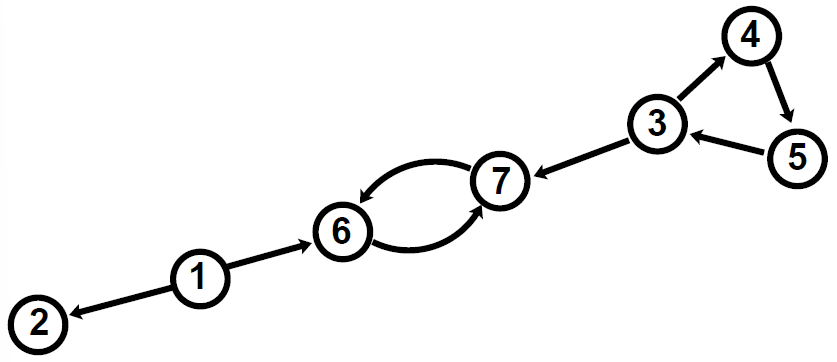
\includegraphics[width=0.5\textwidth]{digrafPrimjer.png}
    \caption{Primjer grafa $G_1$}
    \label{fig:Pr1}
\end{figure}

\begin{exa}
    Pogledajmo primjer grafa $G_1$ sa slike \ref{fig:Pr1} preuzetoga iz \cite{DiGraphReach}:  
Ovdje svaki doseg ima jedan neprazan kabal. Ovaj graf ima dva dosega $R_1 = \{1,2,6,7\}$ i $R_2 = \{3,4,5,6,7\}$ (vidi sliku \ref{fig:Pr1_dosezi}). Ekskluzivni dijelovi su $H_1 = \{ 1,2\}$, $H_2 = \{3,4,5\}$. Kabali su $B_1 = \{1\}$ $B_2 = \{3,4,5\}$. Zajednički dijelovi su $C_1 = C_2 = \{6,7\}$
\end{exa}
\begin{figure}[H]
    \centering
    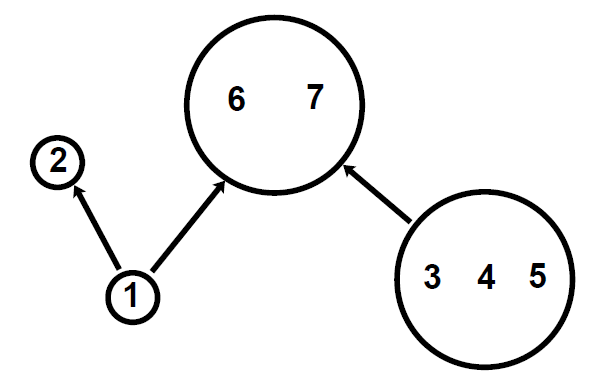
\includegraphics[width=0.5\textwidth]{digrafPrimjer_reaches.png}
    \caption{Dosezi grafa $G_1$}
    \label{fig:Pr1_dosezi}
\end{figure}

Postoji veza između jezgre Laplaceove matrice digrafa $L$ i broja dosega digrafa $G$ \cite{DiGraph_Kernel}:
\begin{thm} %TM 4.6
    Neka je dan digraf G. Tada su algebarska i geometrijska kratnost svojstvene vrijednosti 0 jednake broju dosega. 
\end{thm}
\clearpage
\section[Grafovi u testu][Nekoliko tipova grafova korištenih za testiranje]{Neki tipovi grafova}
U našem radu koristili smo nekoliko vrsta grafova koje nudi Python biblioteka networkx
\subsection{gn\_graph}



%\section[Naslov sekcije u sadržaju][Kratki naslov sekcije]{Naslov sekcije}
\chapter[Uvod u teoriju Multiagentnih sustava][MAS]{Uvod u teoriju Multiagentnih sustava}
\section[Općenito o Multiagentnim sustavima][Općenito o Multiagentnim sustavima]{Općenito o Multiagentnim sustavima}
\subsection{Općenito}
\section[MAS na neusmjerenom grafu][MAS na neusmjerenom grafu]{MAS na neusmjerenom grafu}
Želimo istražiti računanje $H_\infty$ norme MAS ovisno o poemećaju koji se izvrši na jednog agenta ili na skupinu agenata.
U članku \cite{nakic2022short} multiagentni sustav je modeliran kao neusmjereni težinski graf gdje je svaki vrh/agent linearna obična diferencijalna jednadžba drugog reda. Općenito je računanje $H_\infty$ norme MAS-a numerički izuzetno zahtjevno. Uzimajući u obzir strukturu funkcije prijenosa MAS-a može se pokazati da se $H_\infty$ za veliku klasu MAS-a postiže u nuli što bitno pojednostavljuje računanje $H_\infty$ norme te ga proširuje na sustave puno većih dimenzija. 

\subsection{Struktura MAS-a}
Neka je zadano $n$ agenata
\begin{equation}
    \ddot{\chi} = -T_s\dot{\chi} + K_s u_i + \eta_i \omega_i, \qquad T_s, K_s >0
    \label{eq:MAS_ODJ}
\end{equation} gdje su, $\chi_i, u_i$ i $\omega_i$ skalarne funkcije, a $\eta_i$ je faktor smetnje.\\
Funkcija $\chi_i$ predstavlja stanje sustava, $u_i$ predstavlja ulaz, a $\omega_i$ predstavlja izvanjsku smetnju $i$-tog agenta, $i \in \{1,\dots, n\}$.\\
Dinamika agenata \eqref{eq:MAS_ODJ} predstavlja realni dvostruki integrator. Ova dinamika omogućuje posebnije rezultate koje su prikazali u \cite{nakic2022short}.
Široko prihvačen decentraliziran izlazna povratna sprega (eng. output-feedback) koji omogućuje sinkronizaciju mreže je dana u (Ren and Beard (2008 \cite{nakic2022short}) sa:
\begin{equation}
    u_i = -K\hat{C}\sum\limits_{j \in \mathcal{N}_j} w_{ij} \left(\:
    \begin{bmatrix}
        \chi_i \\ \dot\chi_i
    \end{bmatrix}- 
    \begin{bmatrix}
        \chi_j \\ \dot\chi_j
    \end{bmatrix}\right)\:
    \label{eq:feedback}
\end{equation}
gdje su $K>0$ i $\hat{C} = \begin{bmatrix}c_1 & c_2\end{bmatrix}$ sa $c_1, c_2>0$.
Prirodna pretpostavka je da je pripadni neusmjereni graf povezan. Ako nije povezan, može se rastaviti na $k$ samostalnih MAS-a, gdje $k$ označava komponentu povezanosti.

Autori u \cite{nakic2022short} pretpostavljaju da smetnje $\omega_i$ ne moraju sve biti nezavisne, stoga u skupu svih smetnji $\{\omega_1, \dots, \omega_n\}$ pretpostavljaju da ih je $ k \in \{1,\dots,n\}$ različitih $\{\omega_{i_1}, \dots, \omega_{i_n}\}$. Tada je $ \begin{bmatrix}\omega_1, \dots, \omega_n\end{bmatrix}^T = H \begin{bmatrix}\omega_{i_1}, \dots, \omega_{i_n}\end{bmatrix}^T$ gdje je $H \in M_{nk}$ dana s 
\begin{equation*}
    H_{jr} = 
    \begin{cases}
        1, & \omega_j = \omega_{i_r} \\
        0, & \text{inače}
    \end{cases}, j=1, \dots ,n, \quad r = 1,\dots, k.
\end{equation*}
Sa $E = diag(\eta_1,\dots , \eta_n)H \in M_{nk}$ se označi matrica smetnji. Pretpostavlja se da je $\eta_i \neq 0 \text{ ako } H_{ii} \neq 0$ tj. ako se izvrši smetnja $i$-tog agenta, onda pripadna težina nije nula. Iz toga slijedi da je matrica $E$ punog ranga.

Ako se iskoristi da je $L$ Laplaceova matrica neusmjerenog grafa koji pripada MAS-u dinamika zatvorene petlje \eqref{eq:MAS_ODJ} i \eqref{eq:feedback} postaje
\begin{equation}
    \ddot{\chi} + ( \underbrace{T_s}_{:= \beta} I_n + L \underbrace{K_sKc_2}_{:= \alpha} )\dot{\chi} + L \underbrace{K_sKc_1}_{:= \gamma} \chi = E\omega,
    \label{eq:cijeli sustav}
\end{equation}
pritom su $\chi = \left(\chi_1, \dots, \chi_n\right)^T$ i $\omega = \left(\omega_{i_1}, \dots, \omega_{i_n}\right)^T$.

\subsection{Funkcija prijenosa MAS-a}
U prvom koraku cilj je doći do formule za funkciju prijenosa $F(s)= \tilde{C}(is - \tilde{A})^{-1}\tilde{B}$. Pokaže se da je ona oblika:
\begin{align}
    F(0) = \frac{1}{\gamma}L^{+}E, \qquad s=0\\
    F(s) = \frac{1}{\gamma+is\alpha}V V^T (L- qmu(s) I_n)^{-1}E, \qquad s \neq 0
\end{align} pritom su $L^{+}$ Moore-Penroseov pseudoinverz od L i funkcija
$$\mu(s)=\frac{is\beta -s^2}{is \alpha + \gamma} $$

\subsection{Ključan rezultat}
Glavni rezultat je dan u teoremu:
\begin{thm}
    Neka je $\gamma \leq \alpha \beta$ ili ($\gamma > \alpha \beta$ i $||L||\leq \frac{\beta^2}{2(\gamma-\alpha \beta)}$). Tada je
    $$||F||_\infty = {\overline\sigma}(F(0))$$.
\end{thm}

\begin{rem}
    U slučaju da ne vrijedi neki od uvjeta lako se dobiva MAS takav da
    $$||F||_\infty \neq {\overline\sigma}(F(0))$$.
    \textbf{Ubaci neki graf gdje se to vidi.}
\end{rem}


\section[MAS na usmjerenom grafu][MAS na usmjerenom grafu]{MAS na usmjerenom grafu}



\section[MAS numerička implementacija][MAS numerička implementacija]{MAS numerička implementacija}
 $\alpha, \beta, \gamma$
output. funkcija ovisna o parametru $s$:  $$\mu(s)=\frac{is\beta -s^2}{is \alpha + \gamma} $$Računamo 
vrijednost funkcije $F_i(s)$:
\begin{align*}
         F_i(s)  & = \frac{1}{is\alpha + \gamma}VV^T(L-\mu(s)I)^{-1}e_i \\
         & = \left[\: L = ZTZ^T \: \right]\\
         & = \frac{1}{is\alpha + \gamma}VV^TZ(T-\mu(s)I)^{-1}Z^*e_i  \\
         & = \left[ \: VV^TZ = VV^T[\:W \:\: V \:] = V \left[\:0 \: \: I\: \right]  \right] \\
         & = \frac{1}{is\alpha + \gamma}\left[\:0_{n×k} \:\: V \:\right](T-\mu(s)I)^{-1}Z^*e_i\\
         & = \left[\: Z^*e_i = [Z_0 Z_1]^T, \: \: Z_0 \in M_{k,1}, Z_1 \in M_{n-k,1}\: \right]\\
         & = \frac{1}{is\alpha + \gamma} V (T_{22} - \mu(s)I)^{-1} Z_1
\end{align*}
Za $L$ koristimo Schurovu dekompoziciju za $L= ZTZ^T$, $Z= [\: W\:\: V\:],$ $ \: W \in M_{n,k},$ $ \: V \in M_{n,n-k},$ gdje su V stupci od $Z$ koji pripadaju ne-nul elementima i dolazimo do oblika za $\Phi$ (jer vrijedi $L = L V V^T$):

$$\Phi(s) = \left(is \alpha + \gamma \right)\left(\frac{is\beta -s^2}{is \alpha + \gamma}I +L\right) = \\ =  (is \alpha + \gamma)\left(L - \mu(s)I\right),$$
gdje je $\mu(s) =\frac{is\beta -s^2}{is \alpha + \gamma} $.

Za vrijednost u $0$:
$$F_i(0) = \frac{1}{\gamma}V(V^TLV)^{-1}V^Te_i,$$ iskoristi se Schur za L i def za V pa se dobije
$$F_i(0) = \frac{1}{\gamma}VT_{22}^{-1}V^Te_i, $$
gdje je $$ T = 
\begin{bmatrix}
  T_{11} & T_{12}\\
  0 & T_{22}
  \end{bmatrix}.
$$ Pritom blok matrica $T_{11} \in M_{k,k}$ na dijagonali ima $0$, a $T_{22} \in M_{n-k,n-k}$ ima ne-nul svojstvene vrijednosti.





% Na kraju diplomkog rada stavlja se  bibliografija
% Najprije definiramo nacin prikazivanja bibliografije, u ovom slucaju verzija amsplain stila
\bibliographystyle{babamspl} % babamspl ili babplain

% U datoteku diplomski.bib se stavljaju bibliografske reference
% Bibliografske reference u bib formatu se mogu dobiti iz MathSciNet baze, Google Scholara, ArXiva, ...
\bibliography{diplomski}

\pagestyle{empty} % ne zelimo brojanje sljedecih stranica

% I na koncu idu sazeci na hrvatskom i engleskom

\begin{sazetak}
Ukratko ...
\end{sazetak}

\begin{summary}
In this ...
\end{summary}

% te zivotopis

\begin{cv}
Dana ...
\end{cv}

\end{document}